
\vspace{-0.5cm}
\section*{Results}
\vspace{-0.5cm}

In both anisotropic and tuned anisotropic networks, reciprocally
connected pairs occur more often than in a random network with the
same connection density (Fig.~\ref{fig:2neuron1}A).

\begin{center}\vspace{0.01cm}
  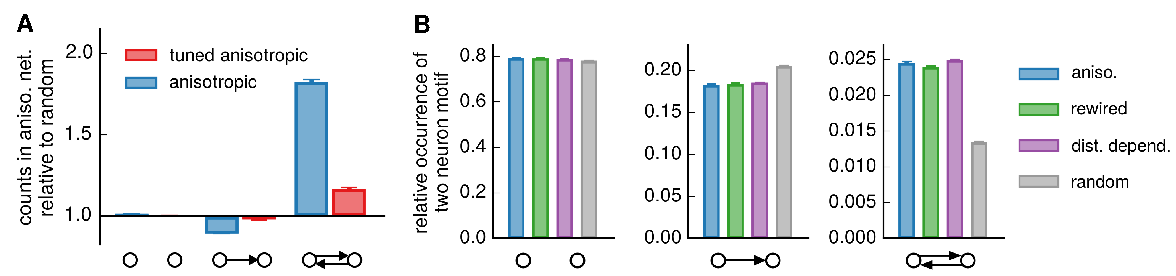
\includegraphics[width=\columnwidth]{%
    figures/two_neuron_figure_part1.pdf}
  \captionof{figure}{Unconnected, unidirectional and bidirectional
    neuron pair occurrences in the network models}
  \label{fig:2neuron1}
\end{center}\vspace{2cm}

However, is this due to anisotropy? Indeed, we find almost identical
pair counts in rewired and distance-dependent networks
(Fig.~\ref{fig:2neuron1}B). The overrepresentation of reciprocal
connections in the data of Perin et al.~\cite{Perin2011} is not
explained by distance-dependency (Fig.~\ref{fig:2neuron2}), so that
there could be other pair-symmetric irregularities in the connection
probabilities that cause the overrepresentation \cite{Hoffmann2017}.

% \begin{center}\vspace{0.01cm}
%   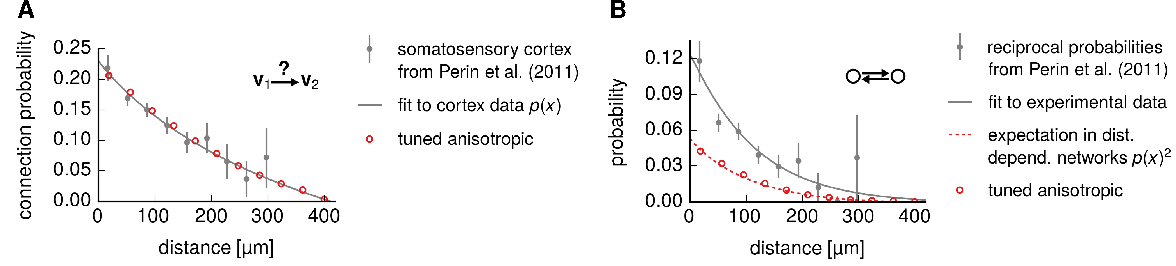
\includegraphics[width=\columnwidth]{%
%     /home/fh/sci/rsc/aniso_netw/pub/arxiv18/figures/two_neuron_connections/two_neuron_figure_part2.pdf}
%   \captionof{figure}{Distance-dependent probability of connection
%     (\textbf{A}) and probability of a reciprocal connection
%     (\textbf{B}).}
%   \label{fig:2neuron2}
% \end{center}\vspace{1.6cm}

Next we tested the occurrence of three neuron patterns as reported in
\cite{Song2005}. We found that in alignment with experimental results,
certain motifs are strongly overrepresented in the anisotropic
networks (Fig.~\ref{fig:3neuron}). Here, it is indeed anisotropy that
causes the motifs to appear more often -- the motif
overrepresentations are drastically reduced in rewired and
distance-dependent
networks.  %% In particular, motifs 4, 10, 12 and 14 were also reported in \cite{Perin2011} to be overrepresented.

\begin{center}\vspace{0.01cm}
  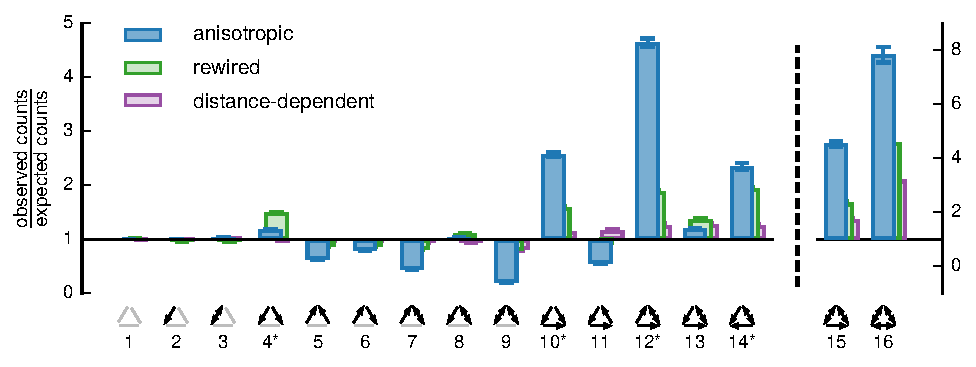
\includegraphics[width=\columnwidth]{%
    figures/fig4_3motif_aniso-rew-dist.pdf}
  \captionof{figure}{Occurrence of three neuron patterns relative to
    expected counts from pair statistics. Motifs indexed with * were
    reported to be overrepresented in \cite{Perin2011}.}
  \label{fig:3neuron}
\end{center}\vspace{2cm}

Perin et al.~\cite{Perin2011} reported that in somatosenory cortex of
rats, groups of neurons more often show a high connection density than
expected from the measured distance-dependent connection
probabilities. Both anisotropic and tuned anisotropic networks also
showed this effect in groups of 3, 6, 8 and 12 cells
(Fig.~\ref{fig:clusters}).

\begin{center}\vspace{0.01cm}
  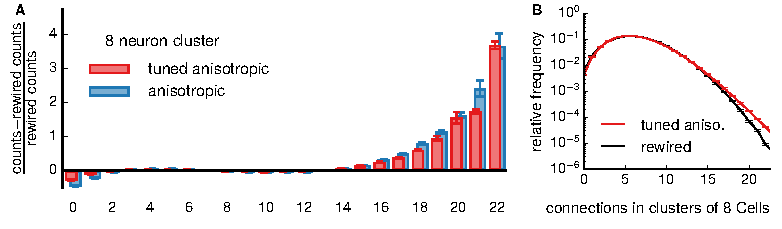
\includegraphics[width=\columnwidth]{%
    figures/nc2_8c-8f.pdf} \captionof{figure}{[Image to be updated]
    For groups of 8 cells a high number of connections appears more
    often in anisotropic and tuned anisotropic networks than in their
    rewired versions. \textbf{A} Relative difference in occurrence
    \textbf{B} Frequency of number of connections in anisotropic and
    rewired network.}
  \label{fig:clusters}
\end{center}\vspace{2cm}

What other network connectivity properties does anisotropy affect? By only partially rewiring anisotropic networks, we found that the distribution of shared inputs to a random pair of neurons is shaped by anisotropy (Fig.~\ref{fig:rewcom}).


\begin{center}\vspace{0.01cm}
  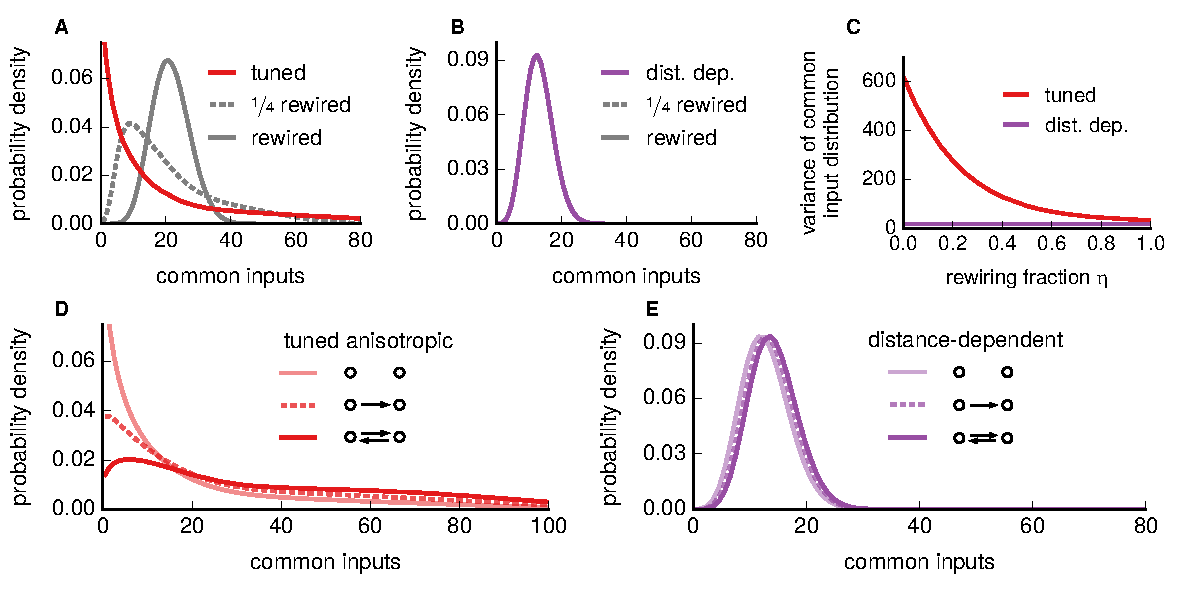
\includegraphics[width=\columnwidth]{%
    figures/fig6.pdf}
  \captionof{figure}{[Image to be updated] \textbf{A} Distribution of
    common in-neighbours to a random neuron pair in anisotropic
    networks ($\eta = 0$) partially rewired networks ($\eta=0.25$) and
    fully rewired networks ($\eta=1$). \textbf{B} Variance of the
    common in-neighbour distribution as a function of the rewiring
    factor.}
  \label{fig:rewcom}
\end{center}\vspace{2cm}





